%\setchapterimage{Fond_SLCI.png}
\setchapterpreamble[u]{\margintoc}
\chapter{Culture algorithmique}

%\marginnote[5cm]{
%\UPSTIcompetence[2]{C1-02}
%\UPSTIcompetence[2]{C2-04}
%}

\section{Intégration numérique}
%\marginnote[4cm]{\textbf{Qui}, \textit{Quoi}, Où.}


\begin{hypo}  $f:[a,b]\rightarrow \mathbb{R}$ est une fonction continue sur $[a,b]$. On note $I = \int\limits_a^{b} f(x) \mathrm{d}x $.
\end{hypo}

\subsection{Principe des méthodes des rectangles}
%\subsection{Principe}
\begin{defi}
Dans cette méthode, la fonction à intégrer est interpolée par un polynôme de degré 0, à savoir une fonction constante. Géométriquement, l'aire sous la courbe est alors approximée par un rectangle. Plusieurs choix sont possibles.

\paragraph*{Rectangles à gauche}
$I = \int\limits_a^{b} f(x) \mathrm{d}x \simeq \left(b-a\right) f(a) $

\paragraph*{Point milieu}
$I = \int\limits_a^{b} f(x) \mathrm{d}x \simeq \left(b-a\right) f\left(\dfrac{a+b}{2}\right) $

\paragraph*{Rectangles à droite}
$I = \int\limits_a^{b} f(x) \mathrm{d}x \simeq \left(b-a\right) f(b) $

\end{defi}

\subsection{Interprétation graphique}

\begin{figure*}[!h]
\begin{minipage}[c]{.24\linewidth}
\begin{center}
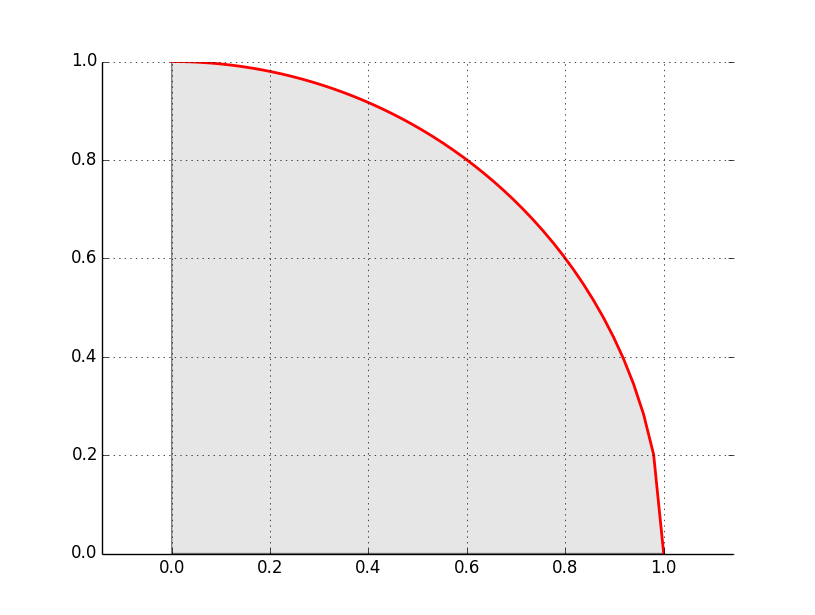
\includegraphics[width=.99\textwidth]{pi_courbe}

\textit{Calcul intégral}
\end{center}
\end{minipage}\hfill
\begin{minipage}[c]{.24\linewidth}
\begin{center}
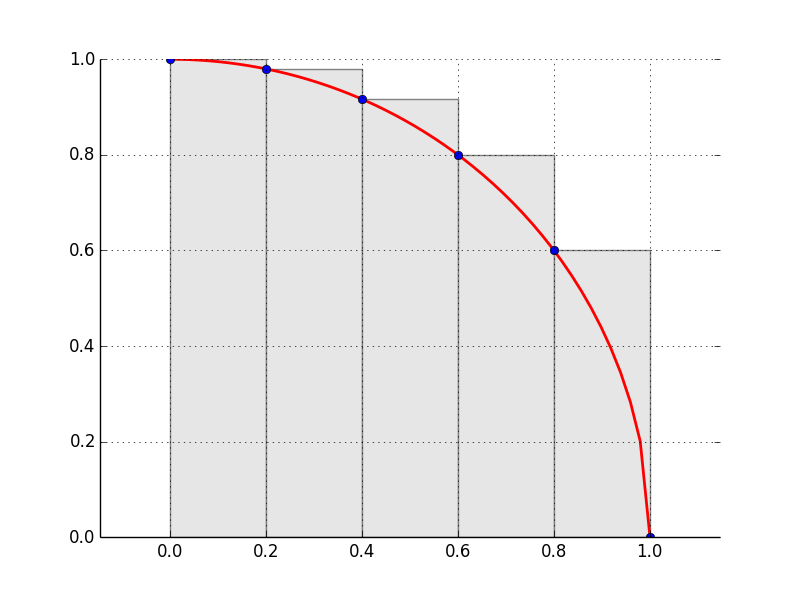
\includegraphics[width=.99\textwidth]{pi_rect_g}

\textit{Rectangles à gauche}
\end{center}
\end{minipage}\hfill
\begin{minipage}[c]{.24\linewidth}
\begin{center}
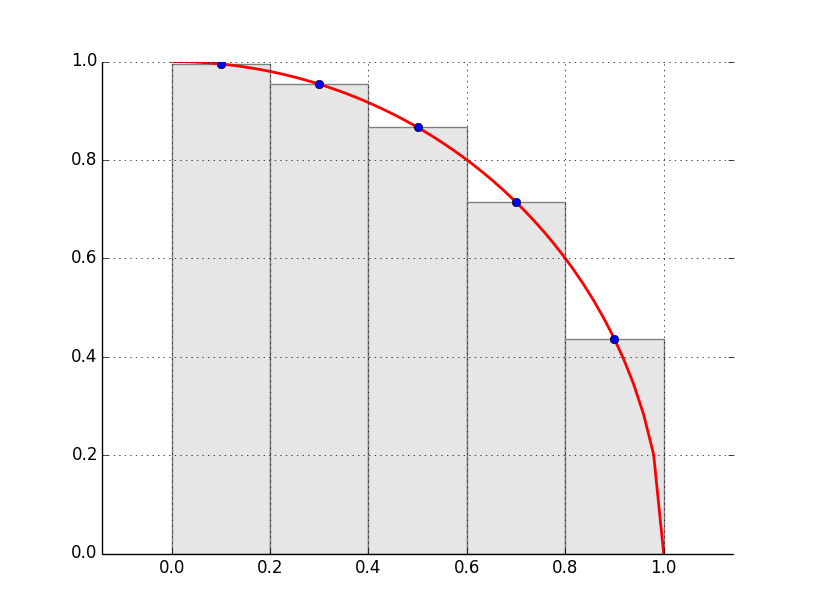
\includegraphics[width=.99\textwidth]{pi_rect_m}

\textit{Point milieu}
\end{center}
\end{minipage}\hfill
\begin{minipage}[c]{.24\linewidth}
\begin{center}
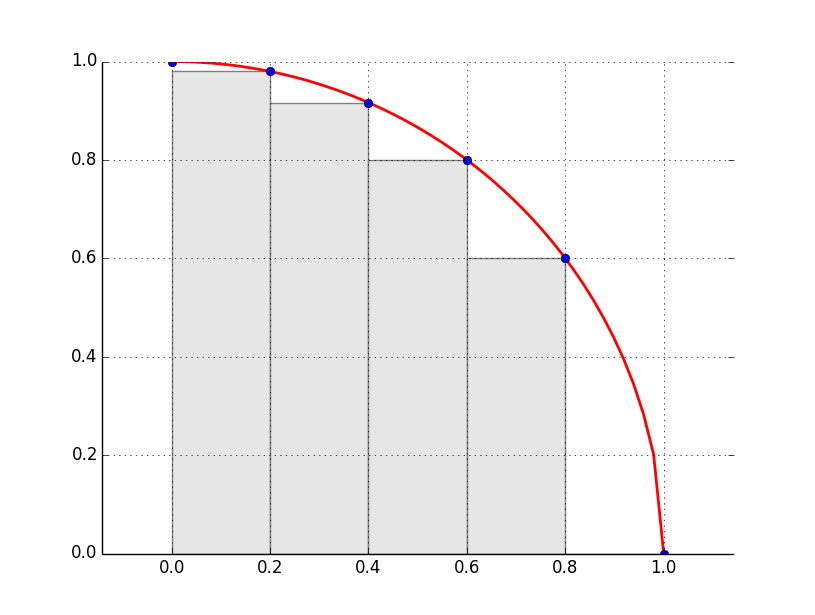
\includegraphics[width=.99\textwidth]{pi_rect_d}

\textit{Rectangles à droite}
\end{center}
\end{minipage}
\end{figure*}

\begin{marginfigure}
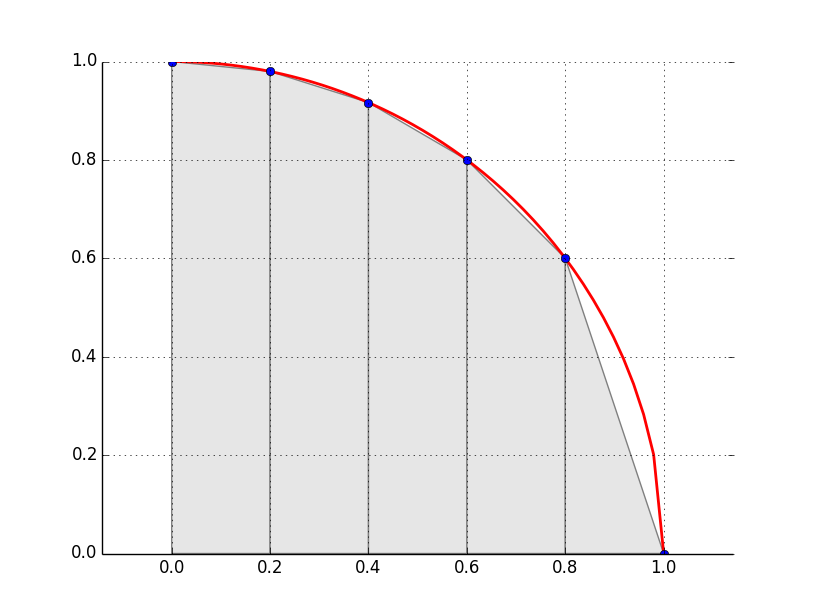
\includegraphics[width=\textwidth]{pi_trap}
\end{marginfigure}

\subsection{Principe des méthodes des trapèzes}


\begin{defi}
Dans cette méthode, la fonction à intégrer est interpolée par un polynôme de degré 1, à savoir une fonction affine. Géométriquement, l'aire sous la courbe est alors approximée par un trapèze :
$I = \int\limits_a^{b} f(x) \mathrm{d}x \simeq \left(b-a\right) \dfrac{f(a)+f(b)}{2} $
\end{defi}


\subsubsection{Notion d'erreur d'intégration}
\begin{resultat}
Dans chaque cas,  on intègre $f$ sur $n$ subdivisions régulières de $I$. 

\textbf{Erreur sur la méthode des rectangles à gauche et à droite}

Soit $f$ fonction dérivable sur $I=[a,b]$ et dont $f'$ est continue sur $I$. Soit $M_1$ un majorant de $f'$ sur $I$. L'erreur $\varepsilon$ commise lors de l'intégration par la méthode des rectangles à droite ou à gauche
 est telle que $ \varepsilon \leq \dfrac{M_1}{2n}$.

\textbf{Erreur sur la méthode des rectangles -- point milieu}

Si de plus $f$ est deux fois dérivables sur $I=[a,b]$ et $f''$ est continue sur $I$, on note $M_2$ un majorant de $f''$ sur $I$.L'erreur $\varepsilon$ commise lors de l'intégration par la méthode des rectangles -- point milieu est telle que $ \varepsilon \leq \dfrac{M_2}{12n^2}$.

\textbf{Erreur sur la méthode des trapèzes}

L'erreur commise$\varepsilon$ est telle qu'il existe un entier $M$ tel que $ \varepsilon \leq \dfrac{M}{12n^2}$.

\end{resultat}


\subsubsection{Bibliothèque Python}
Il est possible d'intégrer une fonction en utilisant les modules de la bibliothèque \texttt{scipy} :
\begin{lstlisting}
from scipy.integrate import quad
from math import sin
# Définition des bornes de gauche et de droite
g,d = -1,1 
def f(x):
    return sin(x)
   
I,erreur = quad(f,g,d)
print(I,erreur)
\end{lstlisting}

\subsection{Implémentation des algorithmes d'intégration}
\subsubsection{Méthode des rectangles à gauche}

\begin{lstlisting}
def integrale_rectangles_gauche(f,a,b,nb):
    """
    Calcul de la valeur approchée de l'intégrale de f(x) entre a et b par la 
    méthode des rectangles à gauche.
    Keywords arguments :
    f -- fonction à valeur dans IR
    a -- flt, borne inférieure de l'intervalle d'intégration
    b -- flt, borne supérieure de l'intervalle d'intégration
    nb -- int, nombre d'échantillons pour le calcul
    """
    res = 0
    pas = (b-a)/nb
    x = a
    while x<b:
        res = res + f(x)
        x = x + pas
    return res*pas
\end{lstlisting}

\subsubsection{Méthode des rectangles à droite}

\begin{lstlisting}
def integrale_rectangles_droite(f,a,b,nb):
    """
    Calcul de la valeur approchée de l'intégrale de f(x) entre a et b par la 
    méthode des rectangles à droite.
    Keywords arguments :
    f -- fonction à valeur dans IR
    a -- flt, borne inférieure de l'intervalle d'intégration
    b -- flt, borne supérieure de l'intervalle d'intégration
    nb -- int, nombre d'échantillons pour le calcul
    """
    res = 0
    pas = (b-a)/nb
    x = a+pas
    while x<=b:
        res = res + f(x)
        x = x + pas
    return res*pas
\end{lstlisting}

\subsubsection{Méthode des rectangles -- Point milieu}
\begin{lstlisting}
def integrale_rectangles_milieu(f,a,b,nb):
    """
    Calcul de la valeur approchée de l'intégrale de f(x) entre a et b par la méthode du point milieu.
    Keywords arguments :
    f -- fonction à valeur dans IR
    a -- flt, borne inférieure de l'intervalle d'intégration
    b -- flt, borne supérieure de l'intervalle d'intégration
    nb -- int, nombre d'échantillons pour le calcul
    """
    res = 0
    pas = (b-a)/nb
    x = a+pas/2
    while x<b:
        res = res + f(x)
        x = x + pas
    return res*pas
\end{lstlisting}

\subsubsection{Méthode des trapèzes pour le calcul approché d'une intégrale sur un segment}

\begin{lstlisting}
def integrale_trapeze(f,a,b,nb):
    """
    Calcul de la valeur approchée de l'intégrale de f(x) entre a et b par la méthode des trapèzes.
    Keywords arguments :
    f -- fonction à valeur dans IR
    a -- flt, borne inférieure de l'intervalle d'intégration
    b -- flt, borne supérieure de l'intervalle d'intégration
    nb -- int, nombre d'échantillons pour le calcul
    """
    res = 0
    pas = (b-a)/nb
    x = a+pas
    while x<b:
        res = res + f(x)
        x = x + pas
    res = pas*(res+(f(a)+f(b))/2)
    return res
\end{lstlisting}

